% Created 2021-06-30 Wed 06:28
% Intended LaTeX compiler: pdflatex
\documentclass[presentation,bigger]{beamer}
\usepackage[utf8]{inputenc}
\usepackage[T1]{fontenc}
\usepackage{graphicx}
\usepackage{grffile}
\usepackage{longtable}
\usepackage{wrapfig}
\usepackage{rotating}
\usepackage[normalem]{ulem}
\usepackage{amsmath}
\usepackage{textcomp}
\usepackage{amssymb}
\usepackage{capt-of}
\usepackage{hyperref}
\usepackage{listingsutf8}
\usepackage{indentfirst}
\usepackage{breakcites}
\usepackage{paralist}
\usepackage{units}
\usepackage{listings}
\let\itemize\compactitem
\let\description\compactdesc
\let\enumerate\compactenum
\usepackage{tikz}
\usetikzlibrary{arrows.meta}
\usetikzlibrary{positioning}
\usepackage{xmpmulti}
\newcommand{\divides}{\mid}
\newcommand{\notdivides}{\nmid}
\setbeamertemplate{footline}[frame number]
\usetheme{default}
\author{Murray Fordyce}
\date{\today}
\title{Snake AI \& Testing Framework}
\subtitle{"What I Did on My Summer Holiday"}
\hypersetup{
 pdfauthor={Murray Fordyce},
 pdftitle={Snake AI \& Testing Framework},
 pdfkeywords={},
 pdfsubject={},
 pdfcreator={Emacs 27.2 (Org mode 9.4.6)}, 
 pdflang={English}}
\begin{document}

\maketitle

\section{Presentation}
\label{sec:org9337e65}
\begin{frame}[label={sec:orgd1e2826}]{Abstract}
\begin{block}{Original Goals}
\begin{itemize}
\item Quantitative Analyses of Different AI Strategies
\end{itemize}
\end{block}
\begin{block}{Background}
\begin{itemize}
\item What is Snake
\item Motivation
\end{itemize}
\end{block}
\begin{block}{Design - Chronological}
\begin{itemize}
\item Ncurses
\item Snake Game
\item First AI
\item Further AIs and Tools
\end{itemize}
\end{block}
\end{frame}
\begin{frame}[label={sec:org7d5d798}]{What is Snake?}
\begin{center}

\includegraphics[width=.9\linewidth]{./snek-40.png}
\end{center}
\end{frame}
\begin{frame}[label={sec:orgc15e6e0}]{Motivation}
\begin{block}{XKCD 356 - Nerd Sniping}
\begin{center}
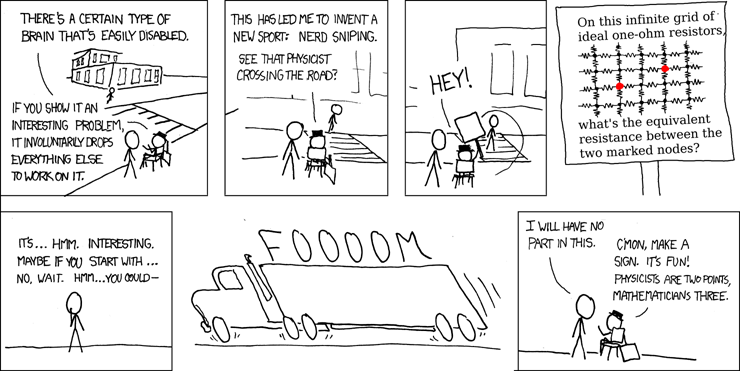
\includegraphics[width=.9\linewidth]{./nerd_sniping.png}
\end{center}
\end{block}
\end{frame}
\begin{frame}[label={sec:orgcbca53d}]{Ncurses (Console Graphics)}
\begin{itemize}
\item Familiar
\item Previous Project (\color{blue}\href{https://github.com/unDeadHerbs/Console-IO}{Github}\color{black})
\item Not Event Based
\end{itemize}
\end{frame}
\begin{frame}[label={sec:org7c52473}]{The Game Class}
\begin{block}{Data}
\begin{itemize}
\item Board Size
\item Snake Length
\item List of Body Points
\item List of Pre-Rendered Body "Tiles"
\item Apple Location
\item Game Ticks
\end{itemize}
\end{block}
\begin{block}{Methods}
\begin{itemize}
\item Render
\item Move
\end{itemize}
\end{block}
\begin{block}{Other}
\begin{itemize}
\item Enum for directions
\end{itemize}


\begin{flushright}
\color{blue}\href{https://github.com/unDeadHerbs/Snek\_player/blob/master/snek\_game.hpp}{GitHub}
\end{flushright}
\end{block}
\end{frame}
\begin{frame}[label={sec:orgb45ae64}]{First AI}
\begin{block}{Using A*}
\begin{itemize}
\item Canonical Search Algorithm
\item Simple
\item Test The Framework
\item Surprisingly Good
\end{itemize}


\vfill
\vfill
\begin{flushright}
\color{blue}\href{https://github.com/unDeadHerbs/Snek\_player/blob/79c6553/snek\_main.cpp\#L62}{GitHub}
\end{flushright}
\end{block}
\end{frame}
\begin{frame}[label={sec:orgc2eb8fe}]{Further AIs and Tools}
\begin{block}{Generalized Tree Search}
\begin{itemize}
\item Cost Metrics
\item Early Cutting
\end{itemize}
\end{block}
\begin{block}{Tools to Inspect AI}
\begin{itemize}
\item Plan Map
\item Logging Framework
\end{itemize}
\end{block}
\begin{block}{Collection of Metrics}
\begin{itemize}
\item Inspection of Game's State (AI Agnostic)
\item Isolated in Driver
\end{itemize}
\end{block}
\end{frame}
\begin{frame}[label={sec:org827db76}]{Distractions, Biases, and Future Work}
\begin{block}{Distractions}
\begin{itemize}
\item Making a Single Better AI
\end{itemize}
\end{block}
\begin{block}{Biases}
\begin{itemize}
\item I Prefer GOFAI
\end{itemize}
\end{block}
\begin{block}{Future Work}
\begin{itemize}
\item Metric for Worst/Average Decision Time
\item Threaded Simulation
\item More Simple AIs
\item Adversarial Apple Placement
\end{itemize}
\end{block}
\end{frame}
\end{document}
